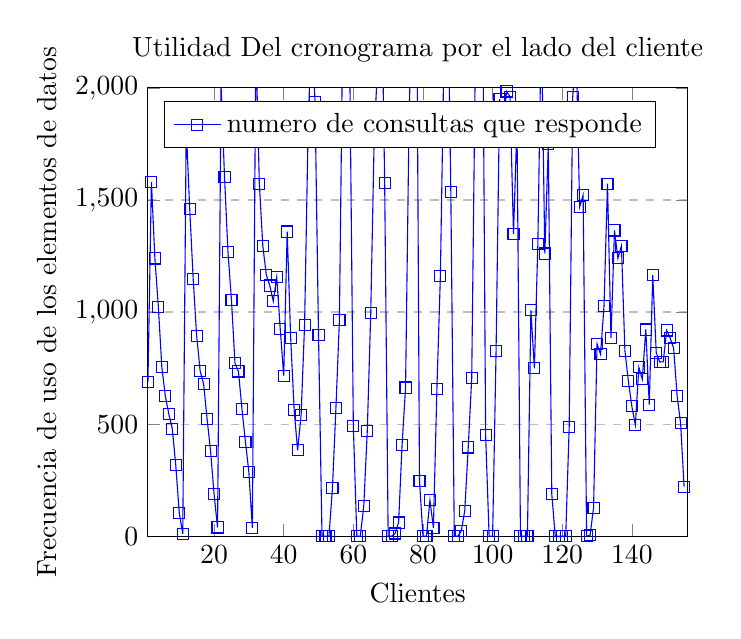
\begin{tikzpicture}
\begin{axis}[
    title={Utilidad Del cronograma por el lado del cliente},
    xlabel={Clientes},
    ylabel={Frecuencia de uso de los elementos de datos},
    xmin=1, xmax=156,
    ymin=0, ymax=2000,
    xtick={},
    ytick={},
    legend pos=north west,
    ymajorgrids=true,
    grid style=dashed,
]

\addplot[
    color=blue,
    mark=square,
    ]
    coordinates {
    %USO EXACTO
    (1,687)
(2,1581)
(3,1239)
(4,1022)
(5,753)
(6,625)
(7,545)
(8,479)
(9,316)
(10,104)
(11,11)
(12,1824)
(13,1461)
(14,1147)
(15,893)
(16,737)
(17,678)
(18,522)
(19,379)
(20,187)
(21,39)
(22,2012)
(23,1603)
(24,1266)
(25,1052)
(26,772)
(27,735)
(28,569)
(29,422)
(30,285)
(31,37)
(32,2208)
(33,1573)
(34,1295)
(35,1166)
(36,1118)
(37,1049)
(38,1156)
(39,925)
(40,716)
(41,1359)
(42,885)
(43,563)
(44,383)
(45,542)
(46,944)
(47,1808)
(48,2299)
(49,1938)
(50,898)
(51,0)
(52,0)
(53,0)
(54,215)
(55,573)
(56,963)
(57,2333)
(58,2244)
(59,2065)
(60,491)
(61,0)
(62,0)
(63,135)
(64,468)
(65,997)
(66,1790)
(67,2110)
(68,2581)
(69,1577)
(70,0)
(71,0)
(72,12)
(73,61)
(74,408)
(75,663)
(76,1855)
(77,2501)
(78,3070)
(79,248)
(80,0)
(81,0)
(82,160)
(83,37)
(84,657)
(85,1160)
(86,2130)
(87,2614)
(88,1534)
(89,0)
(90,0)
(91,23)
(92,113)
(93,396)
(94,704)
(95,2082)
(96,2240)
(97,2799)
(98,450)
(99,0)
(100,0)
(101,827)
(102,1951)
(103,1817)
(104,1984)
(105,1961)
(106,1349)
(107,1837)
(108,0)
(109,0)
(110,0)
(111,1008)
(112,749)
(113,1304)
(114,2304)
(115,1261)
(116,1748)
(117,187)
(118,0)
(119,0)
(120,0)
(121,0)
(122,488)
(123,1958)
(124,2177)
(125,1469)
(126,1521)
(127,0)
(128,4)
(129,127)
(130,858)
(131,812)
(132,1027)
(133,1573)
(134,885)
(135,1364)
(136,1240)
(137,1295)
(138,828)
(139,691)
(140,579)
(141,496)
(142,753)
(143,700)
(144,922)
(145,587)
(146,1165)
(147,819)
(148,777)
(149,778)
(150,918)
(151,884)
(152,838)
(153,626)
(154,504)
(155,221)
    };
    \legend{numero de consultas que responde}

\end{axis}
\end{tikzpicture}

